\documentclass[11pt,a4paper]{article}
\usepackage[utf8]{inputenc}
\usepackage{amsmath}
\usepackage{amsfonts}
\usepackage{amssymb}
\usepackage{graphicx}
\usepackage{subcaption}
\graphicspath{ {./figures/} }
\usepackage{lmodern}
\usepackage{array}
\usepackage[left=3cm,right=3cm,top=2cm,bottom=2cm]{geometry}
\title{Bandits on stochastic block-model graphs}
\author{Arthur Mensch, Michaël Weiss}

\DeclareMathOperator*{\prob}{\mathbb{P}}
\DeclareMathOperator*{\expect}{\mathbb{E}}
\DeclareMathOperator*{\cond}{\mathbb{E}_{w|y}}
\DeclareMathOperator*{\condt}{\mathbb{E}_{w|y\propto p_{\theta_t}}}
\DeclareMathOperator*{\set}{\lbrace 1,\dots,K\rbrace}

\begin{document}
\maketitle

\section{Introduction}
\paragraph{}We consider an adversarial multi-arm bandit problem with \textit{side information}. Such a problem, located between \textit{full-information} problem (at each round, the player observe the loss of every arm), and the \textit{bandit problem} (at each round, the player observe only the loss for the arm he choose). It can model several real-life situations, an important one being preference observation on social networks : feeding a user with a given content, we can observe its feedback (\textit{retweet} on Twitter, \textit{like} on Facebook), along with the feedback of some of his friends virally fed with the same content.

The \textit{bandit} problem can be adressed most efficiently using the well-know \verb|Exp3| algorithm, described in \cite{exp3}. Very recently, \cite{valko} has proposed to extend this algorithm to the \textit{side-information problem}, where feedback distribution is modelled using Erdos-Renyi random graphs. Most importantly, this article focuses on ways to estimate loss distribution over arms, not knowing the underlying edge-revelation probability. It draws upper-bounds on maximum expected regret, using methods inspired from geometrical resampling, present in \cite{neu}.

Erdos-Renyi graph are too simple to successfully model social networks, as population clusters leads to non-uniform connection probabilities. More complex models has been proposed for this purpose, including stochastic block models, which extends Erdos-Renyi to graphs with different clusters. We propose an algorithm that extends \verb|DuplExp3| from \cite{valko} to stochastic block models, where bandit cluster label is known. We empirically show that our algorithm outperform \cite{valko} algorithm on any stochastic blockmodel graph with more than $2$ clusters. 

\section{Exp3 on Erdös-Rényi Graph}

\paragraph{}We first recall \cite{valko} settings, and describe the algorithm adapted to Erdös-Renyi graphs, and its underlying principles. The problem is reduced to the situation where all non-chosen arms reveal their loss with unknown probability $r_{11}=r$. This can be modeled by Erdös-Rényi random graphs with parameter $r$: at each step $t$, for all $(i,j)$ node pairs, we construct an edge between $i$ and $j$ with the probability $r$; we observe loss from the neighbours of chosen arm $I_t$.

Erdös-Rényi graph models interaction between a fully-connected group of people, where content is shared with probability $r$. Although it seems very simple, it already requires subtle adaptation of vanilla \verb|Exp3| algorithm for the player to benefit from side-observation.

\subsection{Problem Definition}
We consider a sequential set on iteractions with the multi-armed bandit we assume to have $N$ arms, for each step $t=1,..,T$ these are the actions performed by the environment : 
\begin{enumerate}
\item The environment chooses losses for every arm noted $l_{t,i}$ for the arm $i$ at the step $t$.
\item Following the algorithm we hope would minize as much as possible the regret the player draws an arm $I_t$.
\item The player receives the losse $l_{t,I_t}$.
\item We define $\left(O_t\right)_{_i\in\left[N\right]}$ as the indicative function of observed loss at step $t$. We have:
\begin{align*}
O_{t,I_t}=1 \qquad \forall i \neq I_t,\, O_{t,i} \sim B\left(r\right.)
\end{align*}
$\left(O_t\right)_{_i\in\left[N\right]}$ corresponds to the value of the logic expression $ i \ is\ neighboor\ of\ I_t$ in the Erdös-Rényi random graph drawn at step t.
\item For all $i$ such that $O_{t,i}=1$ the player can observe the loss $l_{t,i}$.
\end{enumerate}
 
We write $p_{t,i}=\mathbb{P}[I_t=i|\mathcal{F}_{t-1}]$ where $\mathcal{F}_{t-1}$ corresponds to all the actions and observations the player had until the step t. Then intuitively the probability of observing the loss of the arm $i$ at the step $t$ would be $q_{t,i}=p_{t,i} + (1-p_{t,i})r$ and to use the \textsc{Exp}$3$
the the loss estimate :
\[
\hat{l}_{t,i}=\frac{O_{t,i}l_{t,i}}{q_{t,i}}.
\]
But the main problem resides in the fact that $r$ is unknown so the algorithms presented use tricks to obtain loss estimates such that we keep the property :
\[
\mathbb{E}[\hat{l}_{t,i}|\mathcal{F}_{t-1}]=l_{t,i}
\]
The principal idea is to have access to two \textbf{independant} geometrically distributed random variables $M_t^*$ and $K_{t,i}$ with respective parameters $r$ and $p_{t,i}$, then the variable $G_{t,i}^*=\min\{K_{t,i},M_t^*\}$ is also geometrically distributed with the parameter $q_{t,i}$ previously defined. Then if we have $G_{t,i}^*$ \textbf{independant} of $O_{t,i}$ we can replace in the definition of $\hat{l}_{t,i}$, $\frac{1}{q_{t,i}}$ by $G_{t,i}^*$.

\subsection{DuplExp3 for large values of r}
\paragraph{}We assume $ r\geq \frac{log(T)}{2N}$, which implies that the probability of having no additionnal observations in round t is bounded by $\frac{1}{\sqrt{T}}$.\newline
This algorithm needs two \textsc{Exp3} sub-algorithms, with learning rates $\left(\eta_t\right)$. one for the round when t is even and the other one for the rest so that we can construct independant $M_t^*$ and $K_{t,i}$ and independant $G_{t,i}^*$ and $O_{t,i}$.
For each $t$, the algorithm draws:
\[
p_{t+2,i}\propto w_{t+2,i}= \frac{1}{N} exp\left( -\eta_{t+2} \hat{L}_{t,i} \right)
\]
Where $\hat{L}_{t,i}=\sum_{k=0}^{t/2} \hat{l}_{t-2k,i}$ the cumulative sum of the loss estimates for the arm $i$ for one of the \textsc{Exp3} sub-algorithms.

$M_t^*$, truncated geometrical variable of parameters $r$ is constructed as such : 
For all $i=1,...,N-1$, we define $O_{t,i}^{'}$ as:
\begin{align*}
\forall i<I_{t}\ O_{t,i}^{'}=O_{t,i} \qquad \forall N\geq i>I_{t}\ O_{t,i-1}^{'}=O_{t,i} \\
M_t^* =\min\{1\leq i<N: O_{t-1,i}^{'} =1\}\cup\{N\}
\end{align*}
We also define $K_{t,i}$ as a geometric random variable with parameter $p_{t,i}$ computed a the step $t-2$. The since $M_t$ depends of $O_{t-1}$ and $p_{t,i}$ of $\left(O_k\right)_{k\leq t-2}$ they are obviously independant. That's why we can consider :
\begin{align*}
	G_{t,i}=\min\left(K_{t,i},M_t\right)
\end{align*}
with $G_{t,i}$ independant of $O_{t,i}$. $G_{t,i}$ follows a geometrical law of parameter $p_{t,i}+(1-p_{t,i})r$.

We set the loss estimate as:
\begin{align*}
\hat{l_{t,i}}=G_{t,i}O_{t,i}l_{t,i}
\end{align*}
which, taking the expectation, yields:
\begin{align*}
\expect{\hat{l_{t,i}}}&=\expect{G_{t,i}}\expect{O_{t,i}}\expect{l_{t,i}} \\
&= \frac{1}{p_{t,i}+(1-p_{t,i})r} \left(p_{t,i}+(1-p_{t,i})r\right) \expect{l_{t,i}} \\
&= \expect{l_{t,i}}
\end{align*}
which is ununbiased estimator of $l_{t,i}$, as independance allows us to separate expectation. Setting $\eta_t = $, the following upper-bound on the regret can be drawn, using unbiased estimator $\hat l$:
\[
R_T \leq 4 \sqrt{\left(\frac{T}{r}+N^2\right)\log N}+\sqrt{T}
\]
\subsection{Lower-bounding $r$}
However, a problem remains in this algorithm ; since we don't know a priori what is the value of r, we can't ensure that $ r\geq \frac{log(T)}{2N}$ as did the assumption previously. So we need to find a lower bound on $r$ to know in which case we probably are. The algorithm \verb|Estimate |$\underline{r}$ returns the argument $\underline{r}$ with the following properties : 
\begin{align*}
\mathbb{P} [\underline{r}\leq r]&\geq 1-\frac{1}{\sqrt{T}}\\
\mathbb{P} [\underline{r}=0]&=1-\frac{1}{\sqrt{T}},\ \ if\ r\leq \frac{1}{N}\\
\mathbb{P} [\underline{r}=0]&\leq \frac{1}{\sqrt{T}},\ \ if\ r\geq \frac{2}{N}
\end{align*}
Furthermore, let $\tau$ be the index of the round when \verb|Estimate |$\underline{r}$ terminates, then we have :
\begin{align*}
\expect{[\tau]} & = \frac{4\ log\ T}{N}+\sqrt{T}+1,\ if\ r \leq \frac{1}{N}\\
\expect{[\tau]} & = log\ T \left( \frac{4}{N} + \frac{e}{2} \right) + 2,\ if\ r\geq \frac{2}{N}\\
\expect{[\tau]} & = log\ T \left( \frac{4}{N} + e \right) + 2,\ if\ r \in [1/N,2/N]
\end{align*}

These properties will allow us to run this algorithm in first before running a learning algorithm without increasing too much the expected regret. In this configuration, then we can safely estimate that if :
$$ \underline{r} \geq \frac{log\ T}{N} $$
Then we can consider that r is probably large enough to run the previously algorithm \textsc{DuplExp3} on the graph. We will now see how we should proceed in the other cases.

\subsection{Generalized algorithm}
\paragraph{}We now are able to generate a safe lower bound of $r$, $\underline{r}$. This is the first step of the algorithm. We already explained that we could resume to \textsc{DuplExp3} at the current step $\tau$ if we had $ \underline{r} \geq \frac{log\ T}{N}$. We now explain what are the solutions in the other cases.\\

\paragraph{} If $\underline{r}=0$ : \\
We consider that $r$ is really equal to $0$ and run vanilla \textsc{Exp3} with parameter $\eta=\sqrt{\left(2\ log\ N \right)/\left(TN\right)}$ from the step $\tau$.

\paragraph{}If $0< \underline{r} < \frac{log\ T}{N}$ :\\
Then $r$ might be too small so we can have have side information and so have a biased estimation $r$ during the steps. In this case, we use a simple trick to reattach to the case of \textsc{DuplExp3} : The new algorithm groups multiple steps together so that it was as if the number of episodes became,
\begin{align*}
J &= \left\lceil \frac{T}{A} \right\rceil \\
where\ A & =\left\lceil \frac{log T}{N \underline{r}} \right\rceil
\end{align*}
With some adaptations, for instance $I_t$ should be the same for $A$ real rounds and we make sure none of the $O_{t,I_t}$ are counted in the new computation of $M_j$ - where $A(j-1)<t\leq Aj$ which are the grouped steps - and leads less biased estimations of $\hat{l_{j,i}}$.

\section{Exp3 on Stochastic Block-Model Graphs}

\paragraph{}We consider a multi-armed bandit where the arms are divided up in several classes. Every time the learner chooses an arm, not only does he observes the loss of this arm, but he can also have information about losses of non-chosen arms. We model observation graphs by stochastic block models. We consider that when the learner choose a arm of the class $i$, the other arms of the class $i$ have the probability $r_{ii}$ to reveal their loss and the other arms of a class $j$ have the probability $r_{ij}$. The problem is characterized by the matrix $R$ which represents the probabilities of communication between two arms of different classes. In this problem, we assume that the classification of the arm as already been done, so we know the class of each arm and we define $N_i$, the size of the cluster $i$.

\subsection{Problem definition}

As in Sec. 1, everything happens as if, at every time step $t$, we built a stochastic block-model graph, knowing bandit labels. Such graph can model a variety of group interaction, from dissociation to entanglement and layer organisation. We present an example of stochastic block model in Fig \ref{fig:sbm}, with 5 clusters, cluster $i$ being closely connected to cluster $i-1$ and $i+1$ only on the left, and cluster being closely connected from within on the right.

\begin{figure}[ht]
	\centering
	\begin{subfigure}{.49\textwidth}
		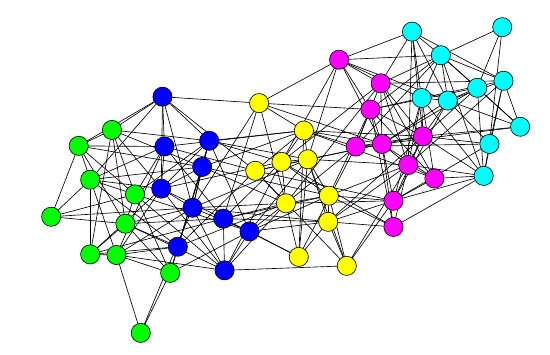
\includegraphics[width=\textwidth]{sbm}
		\caption{ordered communitites}
	\end{subfigure}
	\begin{subfigure}{.49\textwidth}
		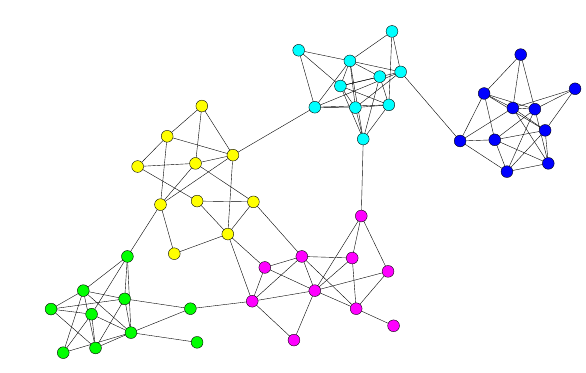
\includegraphics[width=\textwidth]{assortative}
		\caption{Assortative communities}
	\end{subfigure}
	\caption{Stochastic block model random graph (from \cite{sbm})}
	\label{fig:sbm}
\end{figure}

Notations and definition are mostly the same as in Sec. 1, and will be introduced as we adapt \cite{valko} algorithm. 

\subsection{Algorithm}

\paragraph{}\cite{valko} algorithm aims at computing an unbiased estimator for each $(l_{i,t}$, in order to yield satisfying upper bounds on maximum expected regret. We follow the same principle, making use of arms' cluster labels. If we had access to every values $r_{ij}$, we would be able to define, choosing arm $I_t$ at round $t$ : 
\begin{align*}
\hat l_{t,i}^{*} = \frac{O_{t,i}l_{t,i}}{p_{t,i}+(1-p_{t,i})r_{I_t,i}}
\end{align*}
Keeping with the original algorithm, we thus want to build an estimator $G_{i,t}$ that follows a geometrical law of parameter $p_{t,i}+(1-p_{t,i})r_{I_t,i}$. We will rely on the sampling of a geometric variable $M_t$ of parameter $r_{I_t,i}$, making sure that it stays independent from $O_{t,i}$. That way, setting
\begin{align*}
\hat{l_{t,i}}=G_{t,i}O_{t,i}l_{t,i}
\end{align*}
we obtain the desired unbiased estimator. The whole difficulty thus rely on the sampling of $M_t$ so that it stays independent of $O_t$.

\paragraph{$M_t$ sampling}


\subsection{Adaptation of Estimate r, generalized algorithm}
\paragraph{}We now want to provide lower-bounds for every $r_{ij}$ so we know if at a step $t$, after choosing $I_t$ if we need to group so steps to have unbiased loss estimates. This could be done considering $\underline{r}_N^{*}=\min_{j,\ \underline{r}_{i,j}>0}\ \underline{r}_{i,j}\:N_j$ and then using to group the next rounds $A^{*} =\left\lceil \frac{log T}{\underline{r}_N^{}*} \right\rceil$, but would make depend $A^{*}$ of $I_t$ and so might change the number of steps we group at each round. To have a general $A$ which would not depend of $I_j$ we chose at round $j$ we consider :
\begin{align*}
\underline{r}_N^* &= \min_{i,j,\ \underline{r}_{i,j}>0} \underline{r}_{i,j}\:N_j\\
A &= \left\lceil \frac{log T}{\underline{r}_N^{*}} \right\rceil
\end{align*}
Then we can group $A$ steps for each rounds and apply the previously described algorithm.

\paragraph{If $\underline{R}=0$ : \\}
Then we 
\end{document}